\section{Results}\label{sec:results}
We report results by research question. Each subsection ends with a boxed answer that states what the executed evidence supports and what remains open.

\subsection{RQ1: Admission decisions}\label{sec:rq1}
\paragraph{Mutation study.} Table~\ref{tab:local} and Figure~\ref{fig:faults}a derive from the archived \code{decisions.csv}. Direct admission blocks no injected fault. Static validation blocks the \StaticBlocked{} variants of the two graph-fault families (16.7\%), and the smoke proxy additionally blocks the \SmokeAdditional{} process-failure variants (25.0\%). Full readiness blocks all \MutationFaultCases{} faulty variants and admits all \MutationCleanCases{} clean controls. No policy produces a false block, so this suite exhibits no detection/availability trade-off within its narrow valid envelope.

\begin{table}[t]
\caption{Mutation study outcomes per policy. Admitted faults are invalid fixture records accepted by a policy, not observed production failures. False blocks use \MutationCleanCases{} clean controls; seed variants are not independent artifacts.}\label{tab:local}
\centering\small\begin{tabular}{lrrrr}
\toprule Policy & \shortstack{Blocked\\faults} & \shortstack{Admitted\\faults} & \shortstack{Detection\\(\%)} & \shortstack{False\\blocks} \\
\midrule
Direct & 0/240 & 240/240 & 0.0 & 0/20 \\
Static & 40/240 & 200/240 & 16.7 & 0/20 \\
Smoke proxy & 60/240 & 180/240 & 25.0 & 0/20 \\
RES-AI & 240/240 & 0/240 & 100.0 & 0/20 \\
\bottomrule
\end{tabular}

\end{table}

\begin{figure}[t]
\centering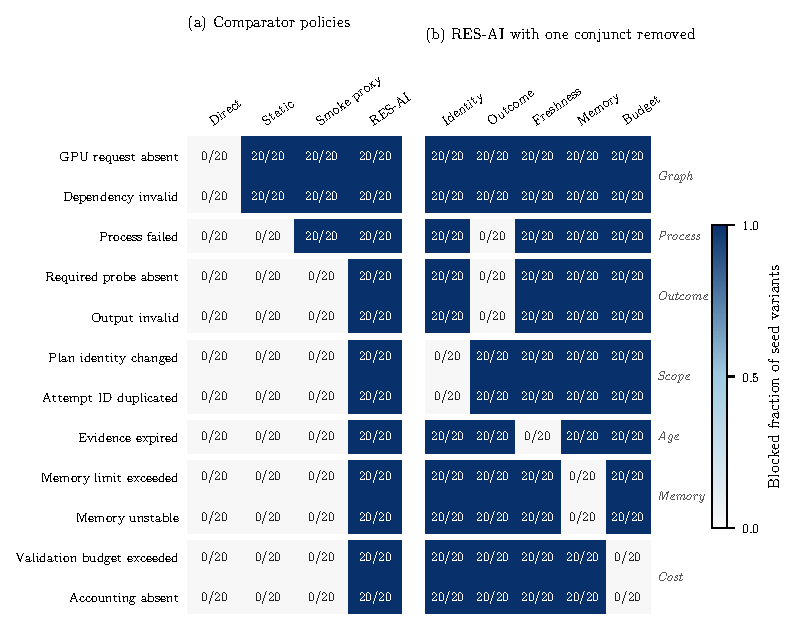
\includegraphics[width=\textwidth]{generated/fault_detection.pdf}
\caption{Blocked variants per fault family, out of \LocalSeeds{} seeds. (a) Comparator policies of the mutation study. (b) Full \tool{} with one conjunct of Equation~\eqref{eq:ready} removed (RQ4). Italic labels group families by the contract concern they violate. Each removed conjunct reopens exactly the families it alone detects.}\label{fig:faults}
\end{figure}

The per-family view (Table~\ref{tab:operators}) explains the aggregate difference. Records with incomplete probe coverage, invalid but present outputs, a changed plan identity, expired evidence, memory violations or invalid accounting all pass both the static validator and the smoke proxy, because each of these faults leaves the job graph valid and the process status successful. A malformed but present output illustrates why file presence is useful for dependencies but insufficient for schema and cardinality. Successful observations of an obsolete plan remain useful history without validating a changed plan.

\paragraph{Threshold sensitivity.} Figure~\ref{fig:sensitivity} shows that every decision boundary moves with its declared parameter and with nothing else. Admission drops from 20/20 to 0/20 between the last grid point at or below $T$ and the first above it (panel a), and between charged totals of 1,200\,s and 1,250\,s when $C=1200$\,s (panel d). For memory headroom (panel b), admission decreases gradually because each seed has its own baseline footprint. At a footprint scale of 1.8, 2, 8 and 9 of 20 seeds remain admissible for $m_{\max}=0.8$, $0.9$ and $0.95$. The static validator and the smoke proxy admit every point of every sweep (dotted lines), because none of the swept properties is visible to them. One implementation detail surfaced at the stability boundary (panel c). When $|m_a-m_b|$ equals $\epsilon$ exactly, 7 of 20 seeds pass for $\epsilon=0.05$ and 15 of 20 for $\epsilon=0.1$, because floating-point rounding of the difference decides the tie. Exact-boundary decisions are therefore not reproducible across inputs, and a production deployment should either quantize telemetry or state a tolerance.

\begin{figure}[t]
\centering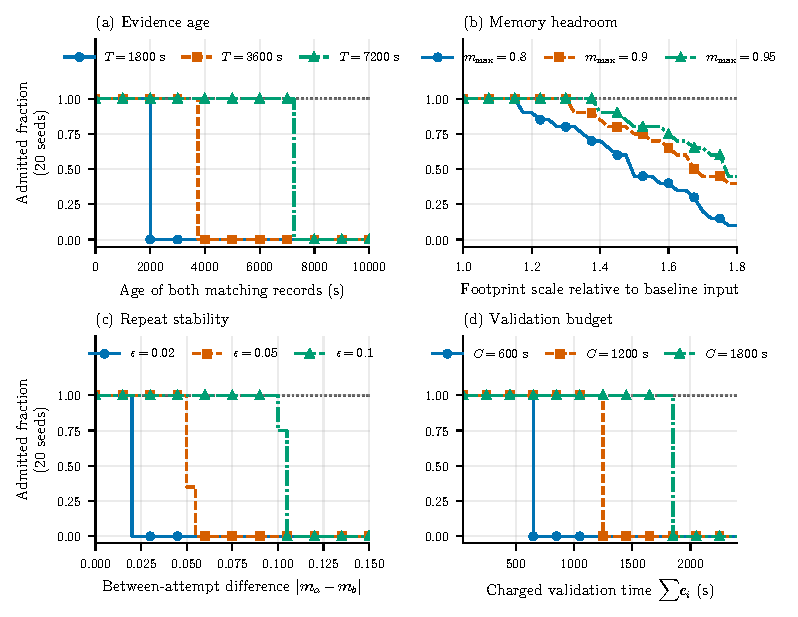
\includegraphics[width=\textwidth]{generated/threshold_sensitivity.pdf}
\caption{Threshold sensitivity of \tool{} admission. Each panel sweeps one evidence property while all other properties remain valid; lines correspond to three settings of the governing parameter and each point aggregates \LocalSeeds{} seeds. The dotted line at 1.0 is shared by the static validator and the smoke proxy, which never respond to these properties. Step lines hold the value until the next grid point.}\label{fig:sensitivity}
\end{figure}

\paragraph{GPU integration.} All eight CUDA probe records were collected from the two completed GPU array cells (job \code{24888989}), and the dependent analysis job \code{24888990} completed. The clean pair passed the retrospective readiness assessment; corrupted-output, missing-checkpoint and runtime-failure pairs were blocked. Slurm reports 81 allocated MIG-instance seconds across the two cells, with 159 seconds of queue delay for each. The timed probe computations sum to 3.723 instance-seconds; the difference includes environment setup, imports and job overhead. These are measurements of this small integration workload, not saved production compute or evidence about an agent's task accuracy.
Table~\ref{tab:gpu} shows that the pilot reproduces two faults that an exit-code check would miss. The corrupt-output processes complete successfully but fail coverage and output validity, and the missing-checkpoint processes produce valid outputs but fail a mandatory obligation. The deliberately raised runtime failure is visible both to status checks and to the readiness rule. Memory headroom is ample in this small workload, so the pilot provides no test of large-model memory pressure.

\begin{table}[t]
\caption{CUDA diagnostics for two repetitions on Nibi. $t_0,t_1$ are timed probe-process seconds. Probes gives the passed obligations out of five in \emph{each} repetition; Output gives valid records out of two. Assessment uses the pair.}\label{tab:gpu}
\small\centering\begin{tabularx}{\textwidth}{lrrccY}
\toprule Mode & $t_0$ (s) & $t_1$ (s) & Probes & Output & Assessment / reasons \\
\midrule
Clean & 0.599 & 0.585 & 5/5 & 2/2 & Ready \\
Corrupt output & 0.619 & 0.334 & 4/5 & 0/2 & Blocked: coverage; output validity \\
No checkpoint & 0.458 & 0.440 & 4/5 & 2/2 & Blocked: coverage \\
Runtime failure & 0.366 & 0.322 & 3/5 & 0/2 & Blocked: process failure; coverage; output validity \\
\bottomrule
\end{tabularx}

\end{table}

\begin{tcolorbox}[rqbox, title={Answer to RQ1}]
On constructed faults, evidence-bound admission blocked all \MutationFaultCases{} faulty variants without false blocks, whereas the smoke proxy blocked 25.0\%. Decision boundaries follow the declared parameters exactly, except for floating-point ties at the stability threshold. On real hardware, \tool{} blocked two fault modes that exit statuses did not reveal. These results establish conformance to the specification, not detection rates for natural faults.
\end{tcolorbox}

\subsection{RQ2: Validation cost and its bounds}\label{sec:rq2}
\paragraph{Measured allocation cost.} Figure~\ref{fig:gpu-cost} separates waiting, allocation and probe computation in the Level B pilot. The two GPU cells start after the same 159-second queue delay and consume 39 and 42 allocated MIG-instance seconds. Their timed probe computations sum to 3.723 seconds across all eight records, so timed computation accounts for under 5\% of the allocated cost. Reporting only the inner computation would understate the cost of this integration check roughly twentyfold. The remainder includes setup, imports and execution overhead; the archive does not support a causal decomposition of it.

\begin{figure}[t]
\centering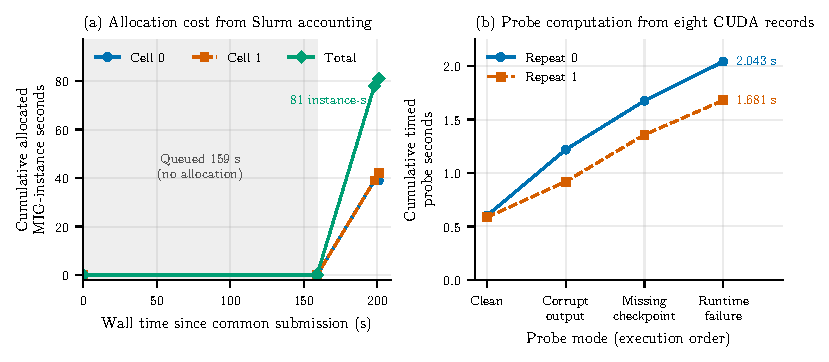
\includegraphics[width=\textwidth]{generated/gpu_cost_timeline.pdf}
\caption{Cost accounting of the Nibi integration pilot. (a) Cumulative allocated MIG-instance seconds reconstructed from Slurm start and end times; queued time accrues no allocated cost. (b) Cumulative timed probe computation in execution order, including the deliberately failing mode. The panels use different accounting boundaries and are not utilization or savings estimates.}\label{fig:gpu-cost}
\end{figure}

\paragraph{Bounded refinement cost.} Figure~\ref{fig:refinement} and Table~\ref{tab:refinement} report the \RefinementEpisodes{} simulated refinement episodes. Charged validation never exceeded the attempt-derived ceiling of $60K$\,s in any episode (Figure~\ref{fig:refinement}b). Mean cost grows with $K$ only until the episodes terminate, then stays flat: additional budget is not consumed once a decision is reached. The cap also limits reachable repairs. With the study setting $K=4$, an initial batch of 64 reached READY in only 2 of 20 episodes, and a batch of 128 in none, because two matching observations plus every failed out-of-memory attempt must fit within $K$. With $K=8$, every initial batch from 16 to 128 converged to READY in the same 14 of 20 episodes, at a mean of 156--336\,s of charged validation. Without declared batch invariance, no proposal was ever produced; episodes that failed with out-of-memory stopped after a single 60-second probe.

\begin{figure}[t]
\centering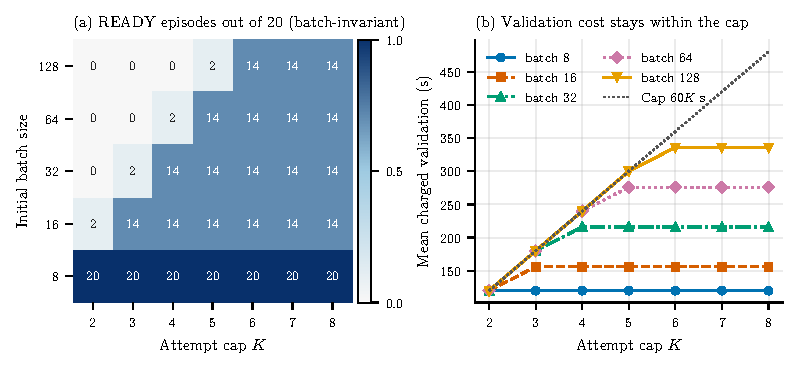
\includegraphics[width=\textwidth]{generated/refinement_bounds.pdf}
\caption{Bounded refinement under the attempt cap $K$ (simulated, batch-invariant contract). (a) Episodes reaching READY out of \LocalSeeds{} seeds by initial batch size and $K$. (b) Mean charged validation time, which never exceeds the $60K$\,s ceiling (dotted) and stops growing once episodes terminate.}\label{fig:refinement}
\end{figure}

\begin{table}[t]
\caption{Terminal decisions of simulated refinement episodes, out of \LocalSeeds{} seeds per row. Ready: READY reached; No prop.: blocked because the contract permitted no further proposal; Cap hit: blocked because the attempt or compute cap was reached; Cost: mean charged validation, with every probe charged 60\,s.}\label{tab:refinement}
\centering\small\setlength{\tabcolsep}{4pt}\begin{tabular}{lrrrrrrrr}
\toprule & \multicolumn{4}{c}{$K=4$ (study setting)} & \multicolumn{4}{c}{$K=8$} \\
\cmidrule(lr){2-5}\cmidrule(lr){6-9} Initial batch & Ready & \shortstack{No\\prop.} & \shortstack{Cap\\hit} & \shortstack{Cost\\(s)} & Ready & \shortstack{No\\prop.} & \shortstack{Cap\\hit} & \shortstack{Cost\\(s)} \\
\midrule
\multicolumn{9}{l}{\emph{Batch-invariant contract}} \\
\quad 8 & 20 & 0 & 0 & 120 & 20 & 0 & 0 & 120 \\
\quad 16 & 14 & 6 & 0 & 156 & 14 & 6 & 0 & 156 \\
\quad 32 & 14 & 6 & 0 & 216 & 14 & 6 & 0 & 216 \\
\quad 64 & 2 & 0 & 18 & 240 & 14 & 6 & 0 & 276 \\
\quad 128 & 0 & 0 & 20 & 240 & 14 & 6 & 0 & 336 \\
\multicolumn{9}{l}{\emph{Batch invariance not declared}} \\
\quad 8 & 20 & 0 & 0 & 120 & 20 & 0 & 0 & 120 \\
\quad 16 & 2 & 18 & 0 & 84 & 2 & 18 & 0 & 84 \\
\quad 32 & 0 & 20 & 0 & 60 & 0 & 20 & 0 & 60 \\
\quad 64 & 0 & 20 & 0 & 60 & 0 & 20 & 0 & 60 \\
\quad 128 & 0 & 20 & 0 & 60 & 0 & 20 & 0 & 60 \\
\bottomrule
\end{tabular}

\end{table}

\paragraph{Assessment overhead.} Figure~\ref{fig:overhead} shows that a readiness assessment costs a median of \OverheadMinMs{}\,ms for a two-record ledger and \OverheadMaxMs{}\,ms for \OverheadMaxAttempts{} records, growing approximately linearly with ledger size. Even at \OverheadMaxAttempts{} records, an assessment costs less than $2\times10^{-4}$ of the shortest measured probe allocation (39\,s). The cost of the gate itself is therefore negligible; the cost of validation lies in the probe allocations it requires.

\begin{figure}[t]
\centering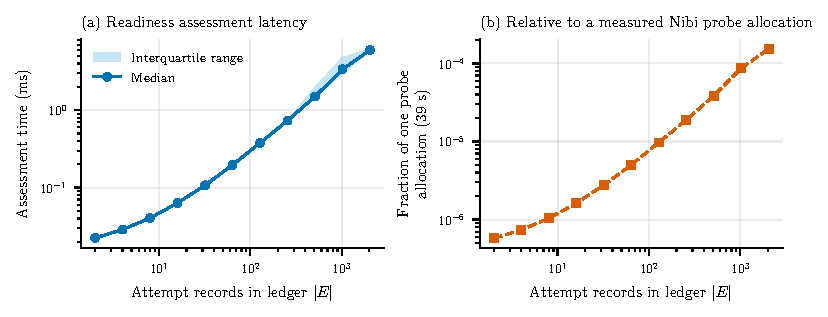
\includegraphics[width=\textwidth]{generated/assessment_overhead.pdf}
\caption{Assessment overhead on the analysis workstation. (a) Median and interquartile range of \OverheadRepeats{} timed calls per ledger size (log--log). (b) The same medians as a fraction of the shortest measured Nibi probe allocation.}\label{fig:overhead}
\end{figure}

\begin{tcolorbox}[rqbox, title={Answer to RQ2}]
Validation cost is dominated by allocations, not by assessment: the pilot's timed computation was under 5\% of its 81 allocated instance-seconds, and the gate costs at most milliseconds. The attempt and compute caps strictly bound charged validation and also limit how many refinements can complete. Whether validation saves resources relative to smoke-then-production remains a campaign question.
\end{tcolorbox}

\subsection{RQ3: Scientific preservation}\label{sec:rq3}
Across the \RefinementEpisodes{} episodes, \tool{} produced \RefinementProposals{} refinement proposals. The hash of the scientific subdocument $S$ was identical before and after each of them (\RefinementScienceChanged{} changes). All proposals came from batch-invariant contracts, and none from contracts without the declaration. This confirms structural preservation: the implementation never rewrites model, data, prompts, seeds or scoring. Structural preservation is necessary but not sufficient for preserving the scientific estimand. Training batch changes can alter optimization, and inference scheduling and numerical nondeterminism can alter outputs.

The initial MapCoder arrays were canceled while pending: first to repair carriage-return configuration defects, then to use the site's documented interactive debugging route after batch admission had no estimated start. A MIG interactive request was also canceled after resource inspection found drained nodes and occupied eligible slices. At the archived status check, full-H100 interactive allocation \code{24890766} was queued for two sequential smoke executions under a separate plan identity. No task-success or readiness result is asserted before collection.
Semantic preservation therefore remains untested by executed evidence; the campaign tests it with equivalence margins fixed before comparison.

\begin{tcolorbox}[rqbox, title={Answer to RQ3}]
No refinement proposal altered the scientific specification, and proposals required an explicit batch-invariance declaration. Whether permitted operational changes preserve experimental outcomes, rather than declared fields, has not yet been measured.
\end{tcolorbox}

\subsection{RQ4: Contribution of contract components}\label{sec:rq4}
Table~\ref{tab:ablation} and Figure~\ref{fig:faults}b show that every conjunct is necessary on this suite. Removing any single component reopens exactly the fault families that only it detects, lowering detection to between 75.0\% (Outcome) and 91.7\% (Freshness). No component is redundant: no family is detected by two different components alone, apart from the graph faults that the upstream validator catches under every variant. Removing a component never introduced false blocks. The Outcome component contributes most because it covers three families, but one of those, process failure, is also caught by the smoke proxy. The components that a successful smoke run cannot replace are therefore identity, freshness, memory and budget, together with coverage and output validity.

\begin{table}[t]
\caption{Leave-one-conjunct-out ablation on the mutation suite (\MutationFaultCases{} faulty and \MutationCleanCases{} clean cases per variant). No variant blocked a clean control.}\label{tab:ablation}
\small\setlength{\tabcolsep}{4pt}\begin{tabularx}{\textwidth}{llrrY}
\toprule Variant & Removed terms of Eq.~(\ref{eq:ready}) & Blocked & Det.\ (\%) & Fault families that escape \\
\midrule
Full \tool{} & none & 240/240 & 100.0 & none \\
$-$Identity & $h_i=h$; distinct IDs &200/240 & 83.3 & Plan identity changed; Attempt ID duplicated \\
$-$Outcome & $\operatorname{OK}$; $O\subseteq C_i$; output &180/240 & 75.0 & Process failed; Required probe absent; Output invalid \\
$-$Freshness & $t-t_i\leq T$ &220/240 & 91.7 & Evidence expired \\
$-$Memory & $m_i\leq m_{\max}$; $\Delta_{\mathrm{smoke}}\leq\epsilon$ &200/240 & 83.3 & Memory limit exceeded; Memory unstable \\
$-$Budget & $|E|\leq K$; $\sum c_i\leq C$; valid $c_i$ &200/240 & 83.3 & Validation budget exceeded; Accounting absent \\
\bottomrule
\end{tabularx}

\end{table}

The refinement study exposes a gap that the ablation cannot. In \HeadroomGapSeeds{} of 20 seeds, halving the batch produced a peak footprint between 0.9 and 1.0 of device capacity (Table~\ref{tab:refinement}, column ``No prop.''). This violates $m_{\max}$ but does not fail with out-of-memory. The Memory conjunct correctly blocks these plans. However, the single implemented refinement fires only on an out-of-memory classification, so it proposes nothing, and the episode stops even though one further halving would satisfy the contract. The memory conjunct and the refinement rule thus use different triggers. Aligning them is a direct improvement for future versions.

\begin{tcolorbox}[rqbox, title={Answer to RQ4}]
Each of the five components of Equation~\eqref{eq:ready} detects fault families that no other component and no smoke check detects, so none can be removed without reopening an escape path. The refinement rule is narrower than the memory conjunct and misses headroom violations that do not fail with out-of-memory.
\end{tcolorbox}
